
\begin{frame}
    \begin{center}
        \LARGE BESDIRAC传输系统
    \end{center}
\end{frame}

\begin{frame}
    \frametitle{BESDIRAC传输系统}
    \begin{itemize}
        \item 目的:为了在网格系统中将数据在高能所及其他站点间进行批量传输。
                考虑到网络环境的不稳定性,需要一个系统监测传输。
        \item 基于DIRAC的Service和Agent,初步开发了基于数据集的传输系统。
        \item 基本的功能
            \begin{itemize}
                \item 数据集的创建
                \item 基于数据集传输请求的创建
                \item 监测特定的传输请求
                \item 可追踪传输过程中的错误信息
            \end{itemize}
        \item 传输系统的架构
            \begin{itemize}
                \item 包含 {Transfer Request Service},
                      {Transfer Agent}及临时的
                      {Dataset Request Service}。
                \item 使用异步I/O实现对传输进程的调度
                \item 抽象 {\tt Transfer Worker},用以支持不同的传输协议
                \item 使用MySQL数据库记录传输的相关信息
            \end{itemize}
    \end{itemize}
\end{frame}

\begin{frame}
    \frametitle{Transfer Agent的设计}
    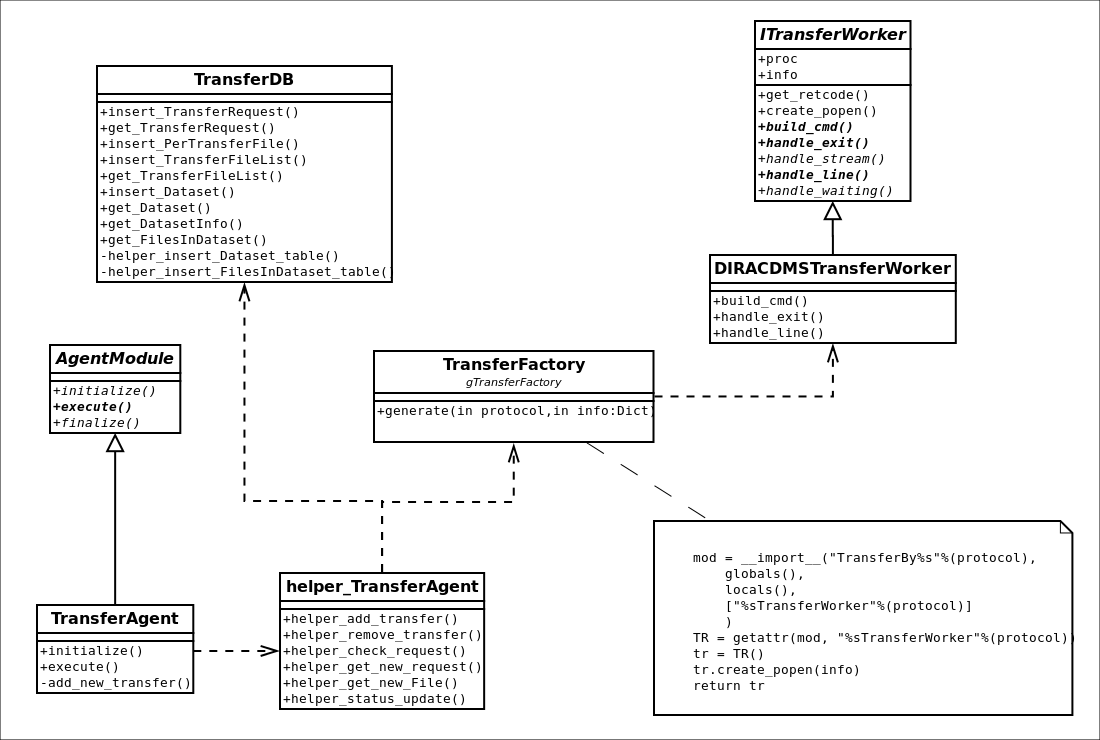
\includegraphics[height=8cm,keepaspectratio]{data/TransferAgent.png}
\end{frame}

